% Created by tikzDevice version 0.10.1 on 2016-08-25 15:40:11
% !TEX encoding = UTF-8 Unicode
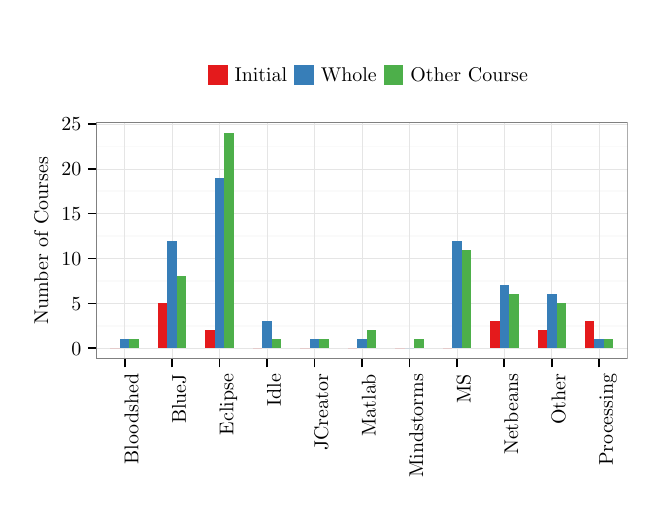
\begin{tikzpicture}[x=1pt,y=1pt]
\definecolor{fillColor}{RGB}{255,255,255}
\path[use as bounding box,fill=fillColor,fill opacity=0.00] (0,0) rectangle (216.81,162.61);
\begin{scope}
\path[clip] (  0.00,  0.00) rectangle (216.81,162.61);
\definecolor{drawColor}{RGB}{255,255,255}
\definecolor{fillColor}{RGB}{255,255,255}

\path[draw=drawColor,line width= 0.6pt,line join=round,line cap=round,fill=fillColor] (  0.00,  0.00) rectangle (216.81,162.61);
\end{scope}
\begin{scope}
\path[clip] ( 24.76, 42.89) rectangle (216.81,128.46);
\definecolor{fillColor}{RGB}{255,255,255}

\path[fill=fillColor] ( 24.76, 42.89) rectangle (216.81,128.46);
\definecolor{drawColor}{gray}{0.98}

\path[draw=drawColor,line width= 0.6pt,line join=round] ( 24.76, 54.88) --
	(216.81, 54.88);

\path[draw=drawColor,line width= 0.6pt,line join=round] ( 24.76, 71.09) --
	(216.81, 71.09);

\path[draw=drawColor,line width= 0.6pt,line join=round] ( 24.76, 87.30) --
	(216.81, 87.30);

\path[draw=drawColor,line width= 0.6pt,line join=round] ( 24.76,103.51) --
	(216.81,103.51);

\path[draw=drawColor,line width= 0.6pt,line join=round] ( 24.76,119.71) --
	(216.81,119.71);
\definecolor{drawColor}{gray}{0.90}

\path[draw=drawColor,line width= 0.2pt,line join=round] ( 24.76, 46.78) --
	(216.81, 46.78);

\path[draw=drawColor,line width= 0.2pt,line join=round] ( 24.76, 62.99) --
	(216.81, 62.99);

\path[draw=drawColor,line width= 0.2pt,line join=round] ( 24.76, 79.19) --
	(216.81, 79.19);

\path[draw=drawColor,line width= 0.2pt,line join=round] ( 24.76, 95.40) --
	(216.81, 95.40);

\path[draw=drawColor,line width= 0.2pt,line join=round] ( 24.76,111.61) --
	(216.81,111.61);

\path[draw=drawColor,line width= 0.2pt,line join=round] ( 24.76,127.82) --
	(216.81,127.82);

\path[draw=drawColor,line width= 0.2pt,line join=round] ( 35.05, 42.89) --
	( 35.05,128.46);

\path[draw=drawColor,line width= 0.2pt,line join=round] ( 52.19, 42.89) --
	( 52.19,128.46);

\path[draw=drawColor,line width= 0.2pt,line join=round] ( 69.34, 42.89) --
	( 69.34,128.46);

\path[draw=drawColor,line width= 0.2pt,line join=round] ( 86.49, 42.89) --
	( 86.49,128.46);

\path[draw=drawColor,line width= 0.2pt,line join=round] (103.64, 42.89) --
	(103.64,128.46);

\path[draw=drawColor,line width= 0.2pt,line join=round] (120.78, 42.89) --
	(120.78,128.46);

\path[draw=drawColor,line width= 0.2pt,line join=round] (137.93, 42.89) --
	(137.93,128.46);

\path[draw=drawColor,line width= 0.2pt,line join=round] (155.08, 42.89) --
	(155.08,128.46);

\path[draw=drawColor,line width= 0.2pt,line join=round] (172.23, 42.89) --
	(172.23,128.46);

\path[draw=drawColor,line width= 0.2pt,line join=round] (189.37, 42.89) --
	(189.37,128.46);

\path[draw=drawColor,line width= 0.2pt,line join=round] (206.52, 42.89) --
	(206.52,128.46);
\definecolor{fillColor}{RGB}{228,26,28}

\path[fill=fillColor] ( 29.90, 46.78) rectangle ( 33.33, 46.78);
\definecolor{fillColor}{RGB}{55,126,184}

\path[fill=fillColor] ( 33.33, 46.78) rectangle ( 36.76, 50.02);
\definecolor{fillColor}{RGB}{77,175,74}

\path[fill=fillColor] ( 36.76, 46.78) rectangle ( 40.19, 50.02);
\definecolor{fillColor}{RGB}{228,26,28}

\path[fill=fillColor] ( 47.05, 46.78) rectangle ( 50.48, 62.99);
\definecolor{fillColor}{RGB}{55,126,184}

\path[fill=fillColor] ( 50.48, 46.78) rectangle ( 53.91, 85.68);
\definecolor{fillColor}{RGB}{77,175,74}

\path[fill=fillColor] ( 53.91, 46.78) rectangle ( 57.34, 72.71);
\definecolor{fillColor}{RGB}{228,26,28}

\path[fill=fillColor] ( 64.20, 46.78) rectangle ( 67.63, 53.26);
\definecolor{fillColor}{RGB}{55,126,184}

\path[fill=fillColor] ( 67.63, 46.78) rectangle ( 71.06,108.37);
\definecolor{fillColor}{RGB}{77,175,74}

\path[fill=fillColor] ( 71.06, 46.78) rectangle ( 74.49,124.57);
\definecolor{fillColor}{RGB}{228,26,28}

\path[fill=fillColor] ( 81.34, 46.78) rectangle ( 84.77, 46.78);
\definecolor{fillColor}{RGB}{55,126,184}

\path[fill=fillColor] ( 84.77, 46.78) rectangle ( 88.20, 56.50);
\definecolor{fillColor}{RGB}{77,175,74}

\path[fill=fillColor] ( 88.20, 46.78) rectangle ( 91.63, 50.02);
\definecolor{fillColor}{RGB}{228,26,28}

\path[fill=fillColor] ( 98.49, 46.78) rectangle (101.92, 46.78);
\definecolor{fillColor}{RGB}{55,126,184}

\path[fill=fillColor] (101.92, 46.78) rectangle (105.35, 50.02);
\definecolor{fillColor}{RGB}{77,175,74}

\path[fill=fillColor] (105.35, 46.78) rectangle (108.78, 50.02);
\definecolor{fillColor}{RGB}{228,26,28}

\path[fill=fillColor] (115.64, 46.78) rectangle (119.07, 46.78);
\definecolor{fillColor}{RGB}{55,126,184}

\path[fill=fillColor] (119.07, 46.78) rectangle (122.50, 50.02);
\definecolor{fillColor}{RGB}{77,175,74}

\path[fill=fillColor] (122.50, 46.78) rectangle (125.93, 53.26);
\definecolor{fillColor}{RGB}{228,26,28}

\path[fill=fillColor] (132.79, 46.78) rectangle (136.22, 46.78);
\definecolor{fillColor}{RGB}{55,126,184}

\path[fill=fillColor] (136.22, 46.78) rectangle (139.65, 46.78);
\definecolor{fillColor}{RGB}{77,175,74}

\path[fill=fillColor] (139.65, 46.78) rectangle (143.08, 50.02);
\definecolor{fillColor}{RGB}{228,26,28}

\path[fill=fillColor] (149.93, 46.78) rectangle (153.36, 46.78);
\definecolor{fillColor}{RGB}{55,126,184}

\path[fill=fillColor] (153.36, 46.78) rectangle (156.79, 85.68);
\definecolor{fillColor}{RGB}{77,175,74}

\path[fill=fillColor] (156.79, 46.78) rectangle (160.22, 82.44);
\definecolor{fillColor}{RGB}{228,26,28}

\path[fill=fillColor] (167.08, 46.78) rectangle (170.51, 56.50);
\definecolor{fillColor}{RGB}{55,126,184}

\path[fill=fillColor] (170.51, 46.78) rectangle (173.94, 69.47);
\definecolor{fillColor}{RGB}{77,175,74}

\path[fill=fillColor] (173.94, 46.78) rectangle (177.37, 66.23);
\definecolor{fillColor}{RGB}{228,26,28}

\path[fill=fillColor] (184.23, 46.78) rectangle (187.66, 53.26);
\definecolor{fillColor}{RGB}{55,126,184}

\path[fill=fillColor] (187.66, 46.78) rectangle (191.09, 66.23);
\definecolor{fillColor}{RGB}{77,175,74}

\path[fill=fillColor] (191.09, 46.78) rectangle (194.52, 62.99);
\definecolor{fillColor}{RGB}{228,26,28}

\path[fill=fillColor] (201.38, 46.78) rectangle (204.81, 56.50);
\definecolor{fillColor}{RGB}{55,126,184}

\path[fill=fillColor] (204.81, 46.78) rectangle (208.24, 50.02);
\definecolor{fillColor}{RGB}{77,175,74}

\path[fill=fillColor] (208.24, 46.78) rectangle (211.67, 50.02);
\definecolor{drawColor}{gray}{0.50}

\path[draw=drawColor,line width= 0.6pt,line join=round,line cap=round] ( 24.76, 42.89) rectangle (216.81,128.46);
\end{scope}
\begin{scope}
\path[clip] (  0.00,  0.00) rectangle (216.81,162.61);
\definecolor{drawColor}{RGB}{0,0,0}

\node[text=drawColor,anchor=base east,inner sep=0pt, outer sep=0pt, scale=  0.72] at ( 19.36, 44.30) {0};

\node[text=drawColor,anchor=base east,inner sep=0pt, outer sep=0pt, scale=  0.72] at ( 19.36, 60.51) {5};

\node[text=drawColor,anchor=base east,inner sep=0pt, outer sep=0pt, scale=  0.72] at ( 19.36, 76.72) {10};

\node[text=drawColor,anchor=base east,inner sep=0pt, outer sep=0pt, scale=  0.72] at ( 19.36, 92.92) {15};

\node[text=drawColor,anchor=base east,inner sep=0pt, outer sep=0pt, scale=  0.72] at ( 19.36,109.13) {20};

\node[text=drawColor,anchor=base east,inner sep=0pt, outer sep=0pt, scale=  0.72] at ( 19.36,125.34) {25};
\end{scope}
\begin{scope}
\path[clip] (  0.00,  0.00) rectangle (216.81,162.61);
\definecolor{drawColor}{RGB}{0,0,0}

\path[draw=drawColor,line width= 0.6pt,line join=round] ( 21.76, 46.78) --
	( 24.76, 46.78);

\path[draw=drawColor,line width= 0.6pt,line join=round] ( 21.76, 62.99) --
	( 24.76, 62.99);

\path[draw=drawColor,line width= 0.6pt,line join=round] ( 21.76, 79.19) --
	( 24.76, 79.19);

\path[draw=drawColor,line width= 0.6pt,line join=round] ( 21.76, 95.40) --
	( 24.76, 95.40);

\path[draw=drawColor,line width= 0.6pt,line join=round] ( 21.76,111.61) --
	( 24.76,111.61);

\path[draw=drawColor,line width= 0.6pt,line join=round] ( 21.76,127.82) --
	( 24.76,127.82);
\end{scope}
\begin{scope}
\path[clip] (  0.00,  0.00) rectangle (216.81,162.61);
\definecolor{drawColor}{RGB}{0,0,0}

\path[draw=drawColor,line width= 0.6pt,line join=round] ( 35.05, 39.89) --
	( 35.05, 42.89);

\path[draw=drawColor,line width= 0.6pt,line join=round] ( 52.19, 39.89) --
	( 52.19, 42.89);

\path[draw=drawColor,line width= 0.6pt,line join=round] ( 69.34, 39.89) --
	( 69.34, 42.89);

\path[draw=drawColor,line width= 0.6pt,line join=round] ( 86.49, 39.89) --
	( 86.49, 42.89);

\path[draw=drawColor,line width= 0.6pt,line join=round] (103.64, 39.89) --
	(103.64, 42.89);

\path[draw=drawColor,line width= 0.6pt,line join=round] (120.78, 39.89) --
	(120.78, 42.89);

\path[draw=drawColor,line width= 0.6pt,line join=round] (137.93, 39.89) --
	(137.93, 42.89);

\path[draw=drawColor,line width= 0.6pt,line join=round] (155.08, 39.89) --
	(155.08, 42.89);

\path[draw=drawColor,line width= 0.6pt,line join=round] (172.23, 39.89) --
	(172.23, 42.89);

\path[draw=drawColor,line width= 0.6pt,line join=round] (189.37, 39.89) --
	(189.37, 42.89);

\path[draw=drawColor,line width= 0.6pt,line join=round] (206.52, 39.89) --
	(206.52, 42.89);
\end{scope}
\begin{scope}
\path[clip] (  0.00,  0.00) rectangle (216.81,162.61);
\definecolor{drawColor}{RGB}{0,0,0}

\node[text=drawColor,rotate= 90.00,anchor=base east,inner sep=0pt, outer sep=0pt, scale=  0.72] at ( 40.00, 37.49) {Bloodshed};

\node[text=drawColor,rotate= 90.00,anchor=base east,inner sep=0pt, outer sep=0pt, scale=  0.72] at ( 57.15, 37.49) {BlueJ};

\node[text=drawColor,rotate= 90.00,anchor=base east,inner sep=0pt, outer sep=0pt, scale=  0.72] at ( 74.30, 37.49) {Eclipse};

\node[text=drawColor,rotate= 90.00,anchor=base east,inner sep=0pt, outer sep=0pt, scale=  0.72] at ( 91.45, 37.49) {Idle};

\node[text=drawColor,rotate= 90.00,anchor=base east,inner sep=0pt, outer sep=0pt, scale=  0.72] at (108.59, 37.49) {JCreator};

\node[text=drawColor,rotate= 90.00,anchor=base east,inner sep=0pt, outer sep=0pt, scale=  0.72] at (125.74, 37.49) {Matlab};

\node[text=drawColor,rotate= 90.00,anchor=base east,inner sep=0pt, outer sep=0pt, scale=  0.72] at (142.89, 37.49) {Mindstorms};

\node[text=drawColor,rotate= 90.00,anchor=base east,inner sep=0pt, outer sep=0pt, scale=  0.72] at (160.04, 37.49) {MS};

\node[text=drawColor,rotate= 90.00,anchor=base east,inner sep=0pt, outer sep=0pt, scale=  0.72] at (177.19, 37.49) {Netbeans};

\node[text=drawColor,rotate= 90.00,anchor=base east,inner sep=0pt, outer sep=0pt, scale=  0.72] at (194.33, 37.49) {Other};

\node[text=drawColor,rotate= 90.00,anchor=base east,inner sep=0pt, outer sep=0pt, scale=  0.72] at (211.48, 37.49) {Processing};
\end{scope}
\begin{scope}
\path[clip] (  0.00,  0.00) rectangle (216.81,162.61);
\definecolor{drawColor}{RGB}{0,0,0}

\node[text=drawColor,rotate= 90.00,anchor=base,inner sep=0pt, outer sep=0pt, scale=  0.72] at (  7.36, 85.68) {Number of Courses};
\end{scope}
\begin{scope}
\path[clip] (  0.00,  0.00) rectangle (216.81,162.61);
\definecolor{fillColor}{RGB}{255,255,255}

\path[fill=fillColor] ( 56.56,137.00) rectangle (185.01,154.07);
\end{scope}
\begin{scope}
\path[clip] (  0.00,  0.00) rectangle (216.81,162.61);
\definecolor{fillColor}{RGB}{228,26,28}

\path[fill=fillColor] ( 65.15,141.98) rectangle ( 72.26,149.09);
\end{scope}
\begin{scope}
\path[clip] (  0.00,  0.00) rectangle (216.81,162.61);
\definecolor{fillColor}{RGB}{55,126,184}

\path[fill=fillColor] ( 96.30,141.98) rectangle (103.41,149.09);
\end{scope}
\begin{scope}
\path[clip] (  0.00,  0.00) rectangle (216.81,162.61);
\definecolor{fillColor}{RGB}{77,175,74}

\path[fill=fillColor] (128.64,141.98) rectangle (135.75,149.09);
\end{scope}
\begin{scope}
\path[clip] (  0.00,  0.00) rectangle (216.81,162.61);
\definecolor{drawColor}{RGB}{0,0,0}

\node[text=drawColor,anchor=base west,inner sep=0pt, outer sep=0pt, scale=  0.72] at ( 74.78,143.06) {Initial};
\end{scope}
\begin{scope}
\path[clip] (  0.00,  0.00) rectangle (216.81,162.61);
\definecolor{drawColor}{RGB}{0,0,0}

\node[text=drawColor,anchor=base west,inner sep=0pt, outer sep=0pt, scale=  0.72] at (105.93,143.06) {Whole};
\end{scope}
\begin{scope}
\path[clip] (  0.00,  0.00) rectangle (216.81,162.61);
\definecolor{drawColor}{RGB}{0,0,0}

\node[text=drawColor,anchor=base west,inner sep=0pt, outer sep=0pt, scale=  0.72] at (138.27,143.06) {Other Course};
\end{scope}
\end{tikzpicture}
